\chapter{SAMBA 4}

O samba 4 vem com a proposta de criar um textit{Active Directory} livre, combatendo as versões pagas da Microsoft, utilizando o LDAP, Bind e Kerberos.

Por se tratar de um sistema ainda em fase de produção e sem previsão para a conclusão atualmente, alguns erros podem aparecer ou alguns parâmetros deverão ser modificados. A versão utilizada nesse trabalho é a Alpha22.

\section{Instalação do SAMBA 4}

Todos os comandos foram testados no Ubuntu 11.04 e Debian 6, por isso algumas adaptações podem ser necessárias em outras distribuições Linux.

A instalação é realizada a partir do terminal, mas antes é necessário a instalação de algumas bibliotecas.

\# apt-get install build-essential libattr1-dev libblkid-dev libgnutls-dev python-dev autoconf python-dnspython git-core

Antes de começar a instalação o relógio do servidor tem que estar atualizado. O comando ntpdate atualiza a hora através do  ntp\footnote[1]{Os servidores NTP permitem aos seus clientes a sincronização dos relógios de seus computadores e outros equipamentos de rede a partir de uma referência padrão de tempo aceita mundialmente, conhecida como UTC (\textit{Universal Time Coordinated}).\cite{RNP}} , onde um dos principais servidores é o br.pool.ntp.org.

\# ntpdate br.pool.ntp.org


%\begin{itemize}
	%\item \textbf{\# ntpdate br.pool.ntp.org} - Atualiza a hora do servidor a partir do servidor br.pool.ntp.org.
%\end{itemize}

O código fonte esta hospedado no servidor git dos desenvolvedores do samba, e o mesmo deve ser clonado para a maquina de destino.

\# git clone git://git.samba.org/samba.git samba-master; cd samba-master

O samba 4 segue os procedimento padrões de instalação de aplicativos no linux através do terminal, que segundo (http://comunidade-linux-brasil.info/content/view/15/3/) se segue com o ./configure, make e o make install.
Nesse caso ao invés de se utilizar o ./configure como padrão é utilizado o ./configure.developer, pois o mesmo habilita alguns modos de debug.

\# ./configure.developer

\# make 

\# make install

Para verificar a versão instalada é só executar o seguinte comando:

\# /usr/local/samba/bin/smbclient "--version 

\section{Criação de Domínio com o Samba 4}

Por padrão o samba 4 é instalado no /usr/local/samba.

\# cd /usr/local/samba

A instalação é a partir da execução do comando provision que fica localizado no /sbin do samba e a inserção de alguns parâmetros.

\# sbin/provision "--use-ntvfs "--realm=NOME\_SERVIDOR "--domain=NOME\_DOMINIO  "--adminpass= Senha12 "--server-role='domain controller'

\begin{enumerate}
	\item \textbf{use-ntvfs} - Habilita o NTVFS\footnote[2]{Sistema de arquivos que armazena os atributos do NTFS};
	\item \textbf{realm} - Domínio do servidor Kerberos;
	\item \textbf{domain} - Domínio do samba;
	\item \textbf{adminpass} - Senha do Administrator, essa senha deve ter pelo menos uma letra maiúscula;
	\item \textbf{server-role} - Regra do servidor.
\end{enumerate}

Depois de instalado e configurado o servidor de textit{Active Directory} pode ser iniciado. Uma das forma é inicia-lo em modo debug para poder acompanhar melhor os processos realizados.

\# /usr/local/samba/sbin/samba -i -M single

Para facilitar a forma de ativar o samba 4 podem ser feito dois procedimentos.

Criar um link do executável do samba no /etc/init.d/

\# ln /usr/local/samba/sbin/samba /etc/init.d/samba

Mudar o caminho da variável de ambiente PATH para que os comandos possam ser acessados fora da sua pasta de origem.

\# echo "export PATH=/usr/local/samba/sbin:/usr/local/samba/bin:\$PATH"  $>$$>$ /root/.bashrc


%\begin{itemize}
%	\item \textbf{\# apt-get install build-essential libattr1-dev libblkid-dev libgnutls-dev python-dev autoconf python-dnspython git-core} - Pacotes necessários para a compilação do samba 4 e download;
%	\item \textbf{\# git clone git://git.samba.org/samba.git samba-master; cd samba-master} - Faz um clone do samba 4 que esta no repositório para o servidor;
%	\item \textbf{\# ./configure.developer} - Configurar as bibliotecas com parâmetros de desenvolvedor. Habilitando alguns modos de debug;
%	\item \textbf{\# make} - Faz uma leitura do comando Makefile;
%	\item \textbf{\# make install} - Executa os comandos configurados para o parâmetro install do arquivo Makefile;
%	\item \textbf{\# /usr/local/samba/sbin/provision "--use-ntvfs "--realm=iff.bomjesus "--domain=iff  "--adminpass= Senha00 "--server-role='domain controller'} - Cria o domínio samba com AD;
%		\begin{enumerate}
%			\item \textbf{use-ntvfs} - Habilita o NTVFS;
%			\item \textbf{realm} - Domínio do servidor Kerberos;
%			\item \textbf{domain} - Domínio do samba;
%			\item \textbf{adminpass} - Senha do Administrator, essa senha deve ter pelo menos uma letra maiúscula;
%			\item \textbf{server-role} - Regra do servidor.
%		\end{enumerate}
%	\item \textbf{\# /usr/local/samba/bin/smbclient "--version} - Mostra a versão do samba;
%	\item \textbf{\# /usr/local/samba/sbin/samba -i -M single} - Inicia o samba 4 com o modo debug;
%	\item \textbf{\#  echo 'ip do servidor iff.bomjesus iff' $>$$>$ /etc/hosts} - Define um nome para o ip do servidor.
%\end{itemize}

\section{Instalação e configuração do BIND9}

O samba 4 já vem pré configurado para trabalhar com BIND9 para ser o servidor DNS nas versões 9.8 e 9.9.
Atualmente a versão do Bind9 no repositório é a 9.7 e com isso são geradas algumas incompatibilidades e para resolver esses problemas é feito o download e a instalação manual da versão 9.9.

\# wget ftp://ftp.isc.org/isc/bind9/9.9.0/bind-9.9.0.tar.gz

Descompactazação do pacote baixado.
 
\# tar -xzvf bind-9.9.0.tar.gz

Entrar no diretório do bind9

\# cd bind-9.9.0

Configuração para a instalação, informando qual o local de instalação e onde ficarão os arquivos de configuração.

\# ./configure "--prefix=/usr/local/bind9 "--sysconfdir=/etc/bind

\# make

\# make install
% *****EXPLICAR O MAKE*****
% 
% *****EXPLICAR MAKE INSTALL*****

Entrar no diretório onde se encontra os arquivos de configuração do bind

\# cd /etc/bind

Com esse procedimento de instalação os arquivos de configuração não são gerados automaticamente, com isso gerando a necessidade de cria-los manualmente.

\# vim named.conf.options

As seguintes configurações devem ser adicionadas.

options \{
	
directory "/usr/local/bind/var/run/named";

tkey-gssapi-keytab "/usr/local/samba/private/dns.keytab" ;

tkey-domain "nome\_do\_realm\_samba";
	
\};

As variáveis adicionadas no arquivos são para:

\begin{itemize}
	\item{directory} -  É o caminho absoluto do seu servidor dns;
	\item{tkey-gssapi-keytab} - Local da chave do dns para conexão com o kerberos;
	\item{tkey-domain} - Nome do Domínio.
%	\item{auth-nxdomain} - ...
%	\item{listen-on-v6} - ...
\end{itemize}

%\begin{itemize}
%	\item \textbf{\# wget ftp://ftp.isc.org/isc/bind9/9.9.0/bind-9.9.0.tar.gz} - Download da versão 9.9 do bind9;
%	\item \textbf{\# tar xzvf bind-9.9.0.tar.gz} - Descompactar o pacote do bind9;
%	\item \textbf{\# cd bind-9.9.0} - Acessar o diretório do bind9 descompactado;
%	\item \textbf{\# ./configure "--prefix=/usr/local/bind9 "--sysconfdir=/etc/bind} - Configurar os parâmentros para a instalação do bind, tais como o local onde vai ser instalado e onde ficarão os arquivos de configuração;
	% \item \textbf{\# make} - Leitura do comando Makefile;
	% \item \textbf{\# make install} - Executa os comandos configurados para o parâmetro install do arquivo Makefile;
	% \item \textbf{\# cd /etc/bind} - Acessar o diretório onde se encontram os arquivos do bind;
	% \item \textbf{\# vim named.conf} - Cria e edita o arquivo. Adicione as linhas abaixo no arquivo;
	% 	\begin{enumerate}
	% 		\item \textbf{include "/etc/bind/named.conf.options";}
	% 		\item \textbf{include "/etc/bind/named.conf.local";}
	% 	\end{enumerate}
	%  		\item \textbf{\# vim named.conf.options}
	% 		\begin{enumerate}
				% \item \textbf{Adicionar no arquivo} - options \{
%       			
%					directory "/var/cache/bind";
%
%					auth-nxdomain no;
%
%					listen-on-v6 \{ any; \};
%					
%					\};
%			\end{enumerate}
%\end{itemize}

O comando provision gera os arquivos de configuração necessários para o funcionamento do samba com o servidor dns.

\begin{itemize}
	\item \textbf{\# vim named.conf.local} -  Adicione a linha abaixo no arquivo;
		\begin{enumerate}
			\item \textbf{include "/usr/local/samba/private/named.conf";}
		\end{enumerate}
\end{itemize}

Com os arquivos named.conf.local e named.conf.options devidamente criados e configurados, deve-se inclui-los no arquivos named.conf

\# vim named.conf

include "/etc/bind/named.conf.local";
include "/etc/bind/named.conf.options";


Como o samba 4 já vem com configurações prontas do bind9 é necessário escolher qual a versão do dns que esta sendo utilizada.

\begin{itemize}
	\item \textbf{\# vim /usr/local/samba/private/named.conf}
\end{itemize}

\begin{figure}[ht]
   	\centering
    \scalebox{1}{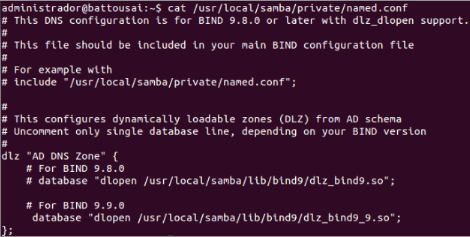
\includegraphics{figuras/named_conf}}
   	\caption{Arquivo named.conf do samba}
    \label{cups}
\end{figure}

% \# For BIND 9.8.0
% 
%     \# database "dlopen /usr/local/samba/lib/bind9/dlz\_bind9.so"; 
% 
% Descomentar
% 
%  \# For BIND 9.9.0
% 
%     database "dlopen /usr/local/samba/lib/bind9/dlz\_bind9\_9.so";

\begin{itemize}
	\item \textbf{\# groupadd named \&\& useradd named -g named} - Cria o usuário responsável pelo bind e o insere no grupo named;
	\item{\# chown named:named /usr/local/samba/private/dns.keytab}
	\item \textbf{\# /usr/local/bind9/sbin/named -u named -g} - Inicia o bind com o usuário named;
\end{itemize}

O servidor samba tem que ter seu endereço DNS configurado para apontar para seu servidor DNS.

\begin{itemize}
	\item \textbf{\# echo 'nameserver ip\_do\_servidor' $>$$>$ /etc/resolv.conf} - Define o endereço do servidor de DNS que o computador irá enviar suas solicitações;
\end{itemize}

A partir de agora para acessar a internet através do servidor samba o bind deverá estar sendo executado.

\section{Instalação do Kerberos}

Segundo \cite{HEIMDAL} a autenticação Kerberos é um protocolo de rede. Foi concebido para fornecer autenticação forte para o cliente/servidores de aplicativos usando criptografia de chaves secretas, então um cliente pode provar a sua identidade para um servidor (e vice-versa) em uma conexão de rede insegura.
Em nosso caso utilizaremos BIND com suporte ao Heimdal Kerberos por causa do GSS-TSIG algoritmo de serviço de segurança genérico para autenticação de transação com chave secreta de DNS (GSS-TSIG) este mecanismo é utilizado para estabelecer relações TSIG para autenticação do tipo Kerberos, necessário para interagir BIND com Samba 4, com essas credenciais o DNS aceita atualizações GSS-TSIG assinadas e verifica as credenciais de correspondentes com as credencias cadastradas no Samba 4, isso permite aos usuários descarregar o DNS dos usuários do Microsoft Windows sem ter a segurança comprometida.

\begin{itemize}
	\item \textbf{\# apt-get install krb5-user krb5-kdc krb5-config kstart} - Instala todos os pacotes necessários e faz as referências necessárias.
\end{itemize}

Após instalar os pacotes, substitua o /etc/krb5.conf pelo arquivo criado e pré-configurado pelo samba que esta localizado em /usr/local/samba/private/krb5.conf

\begin{itemize}
	\item \textbf{\# cp /usr/local/samba/private/krb5.conf  /etc/}
\end{itemize}

Teste para verificar se todos as configurações foram realizadas corretamente

\begin{itemize}
	\item \textbf{\# host -t SRV \_ldap.\_tcp."nome do realm sem aspas".} - O resultado deve ser parecido : \textbf{\_ldap.\_tcp."nome do realm sem aspas" has SRV record 0 100 389 server."nome do realm sem aspas".}
	\item \textbf{\# host -t SRV \_kerberos.\_udp."nome do realm sem aspas".} - O resultado deve ser parecido : \textbf{\_kerberos. \_udp."nome do realm sem aspas" has SRV record 0 100 88 server."nome do realm sem aspas".}
	\item \textbf{\# host -t A "nome do realm sem aspas"} - O resultado deve ser parecido : \textbf{"nome do realm sem aspas" has address "ip do servidor}
\end{itemize}

\section{Kerberos com Bind9}

Configurar atualizações dinâmicas no DNS com o kerberos

Para o funcionamento das atualizações algumas variáveis necessárias de sistema devem ser criadas para o acesso do kerberos com bind

\begin{itemize}
	\item \textbf{\# echo "export KEYTAB\_FILE=/usr/local/samba/private/dns.keytab" >> /root/.bashrc}
	\item \textbf{\# echo "export KRB5\_KTNAME=/usr/local/samba/private/dns.keytab" >> /root/.bashrc}
\end{itemize}

Mudar o dono e o grupo do dns.keytab para que o bind possa alterar o arquivo

\begin{itemize}
	\item \textbf{\# chown named:named /usr/local/samba/private/dns.keytab}
	\item \textbf{\# /usr/local/samba/sbin/samba\_dnsupdate "--verbose} - Atualização automática do dns do samba.
\end{itemize}

\section{Gerenciando o samba 4 no Windows XP}

É possível gerenciar o servidor samba 4 através de um Windows XP mas para a realização do mesmo é necessário a instalação do AdminPack presente no Windows Server.

O AdminPack está disponível no site da Microsoft:  http://www.microsoft.com/downloads/details.aspx?FamilyID=c16ae515-c8f4-47ef-a1e4-a8dcbacff8e3\&displaylang=en 

Com a ferramenta instalada é possível gerenciar todos os usuários, grupos e maquinas presentes no textit{Active Directory}.\ref{tela_dsa}

\begin{figure}[ht]
   	\centering
    \scalebox{1}{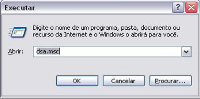
\includegraphics{figuras/dsamsc}}
   	\caption{Tela para executar o DSA}
    \label{dsa}
\end{figure}

\begin{figure}[ht]
   	\centering
    \scalebox{1}{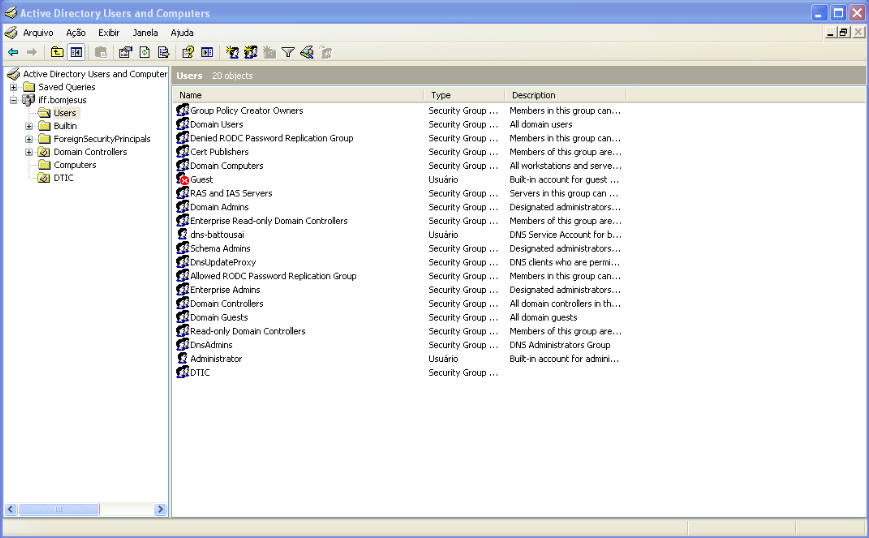
\includegraphics{figuras/addsa}}
   	\caption{Tela do DSA}
    \label{tela_dsa}
\end{figure}


\section{Compartilhamento de arquivos e impressoras}

SAMBA4 ainda não consegue compartilhar arquivos e impressoras de forma fácil e simplificada como o samba 3, e tem problemas com a integração dos usuários e grupos do textit{Active Directory} com os locais, dificultando a definição das permissões a arquivos e diretórios.

Uma solução para tal problema é identificar o código do usuário no textit{Active Directory} e dar as devidas permissões a pasta desejada.

\begin{itemize}
	\item \textbf{\# /usr/local/samba/bin/wbinfo "--name-to-sid USERNAME} - O resultado deve ser o sid do usuário no samba. Exemplo : S-1-5-21-4036476082-4153129556-3089177936-1005 SID\_USER(1)
	\item \textbf{\# /usr/local/samba/bin/wbinfo "--sid-to-uid S-1-5-21-4036476082-4153129556-3089177936-1005} - Mostra o id do usuário e é a referência do usuário local com o do samba 4.
	\item \textbf{\# chown 3000011 /pasta\_que\_será\_compartilhada} - Mudando o usuário do diretório e as suas permissões, o usuário do AD irá ter o acesso aos arquivos.
\end{itemize} 

\section{Gerenciando o Samba4 no Linux}

O samba-tools é uma ferramenta que acompanha o samba 4 e tem a finalidade de gerenciar as ações que podem ser feitas no no textit{Active Directory}. Com ele se poder criar usuários, grupos, gpo's, entre outras funções, porém um forma de texto.

\begin{figure}[ht]
   	\centering
    \scalebox{1}{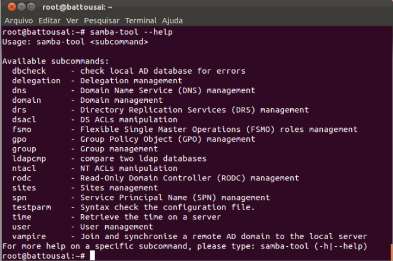
\includegraphics{figuras/samba-tool}}
   	\caption{samba-tool no terminal}
    \label{Samba-tool}
\end{figure}

\section{Maquinas linux e samba3 interagindo com o textit{Active Directory} do  Samba4}

Segundo \cite{UBUNTU-WIKI} a forma de incluir uma maquina Ubuntu no textit{Active Directory} é modificar alguns arquivos de configuração.
Segue abaixo os arquivos e os procedimentos.

\textbf{Informações}

\begin{itemize}
	\item \textbf{fja.br} -  Domínio do textit{Active Directory}
	\item \textbf{fjadc01.fja.br} - Controlador de domínio
	\item \textbf{10.1.0.1} - IP do controlador de domínio
	\item \textbf{FJA.BR} - Kerberos Realm
	\item \textbf{gert} - Estação de Trabalho Ubuntu
	\item \textbf{gert.fja.br} - FQDN da estação de trabalho
	\item \textbf{fjadc01} - Servidor NTP
\end{itemize}

\textbf{Instalando os pacotes necessários}

\begin{itemize}
	\item {\# aptitude install krb5-user libpam-krb5 winbind samba smbfs smbclient krb5-config libkrb53 libkadm55 vim}
\end{itemize}

\textbf{Sincronizando a hora}

\begin{itemize}
	\item {\# ntpdate 10.2.0.1}
\end{itemize}

\textbf{Edite o arquivo /etc/hosts adicionando o ip e o nome do DC de sua rede}

\begin{itemize}
	\item {\# vim /etc/hosts}
\end{itemize}

127.0.0.1       gert.fja.br localhost gert

127.0.1.1       gert

\# The following lines are desirable for IPv6 capable hosts

::1     ip6-localhost ip6-loopback

fe00::0 ip6-localnet

ff00::0 ip6-mcastprefix

ff02::1 ip6-allnodes

ff02::2 ip6-allrouters

ff02::3 ip6-allhosts

10.2.0.1   fjadc01

10.2.0.2   fjadc02

\textbf{Configurando o Kerberos}

\begin{itemize}
	\item {\# vim /etc/krb5.conf}
\end{itemize}

[libdefaults]

	default\_realm = FJA.BR

[realms]

    FJA.BR = \{

      kdc = fjadc01.fja.br

      default\_domain = FJA.BR

      kpasswd\_server = fjadc01.fja.br

      admin\_server = fjadc01.fja.br

     \}

[domain\_realm]

.fja.br = FJA.BR

\textbf {Testando a conexão com o \textit{Active Directory}}

\begin{itemize}
	\item {kinit $<$ENTER$>$}
	\item {Password for alex$@$FJA.BR: ****}
	\item {klist $<$ENTER$>$}
	\item {Ticket cache: FILE:/tmp/krb5cc\_1000}
	\item {Default principal: alex$@$FJA.BR}
\end{itemize}

\textbf {Se o resultado for este o Kerberos está funcionando corretamente}

	Valid starting Expires Service principal 07/16/07 15:48:35  07/17/07 01:49:08  

	krbtgt/FJA.BR@FJA.BR renew until 07/17/07 15:48:35
	
	Kerberos 4 ticket cache: /tmp/tkt1000
	
	klist: You have no tickets cached

\textbf{Acessando o Domínio}

\begin{itemize}
	\item {\# vim /etc/samba/smb.conf} -  Adicione as seguintes linhas
\end{itemize}

[global]

        security = ads

        realm = FJA.BR

        password server = 10.2.0.1

        workgroup = ADMINISTRATIVO

\#       winbind separator = +

        idmap uid = 10000-20000

        idmap gid = 10000-20000

        winbind enum users = yes

        winbind enum groups = yes

        template homedir = /home/\%D/\%U

        template shell = /bin/bash

        client use spnego = yes

        client ntlmv2 auth = yes

        encrypt passwords = yes

        winbind use default domain = yes

        restrict anonymous = 2

\# to avoid the workstation from

\# trying to become a master browser

\# on your windows network add the

\# following lines

        domain master = no

        local master = no

        preferred master = no

        os level = 0

\textbf{Reinicie os serviços}

\begin{itemize}
	\item \textbf{\# /etc/init.d/winbind stop}
	\item \textbf{\# /etc/init.d/samba restart}
	\item \textbf{\# /etc/init.d/winbind start}
\end{itemize}

\textbf{Adicione a conta ao domínio}

\begin{itemize}
	\item \textbf{\# net ads join}
	\item \textbf{Resultado} - Using short domain name – GERT Joined 'GERT' to realm 'FJA.BR'
\end{itemize}

\textbf{Configure a Autenticação}

\begin{itemize}
	\item \textbf{\# vim /etc/nsswitch.conf}
\end{itemize}

	passwd:         compat winbind

	group:          compat winbind

	shadow:         compat

\textbf{Teste o winbind}

\begin{itemize}
	\item {getent passwd}
\end{itemize}

quiosque:*:10018:10000:Quiosque:/home/ADMINISTRATIVO/quiosque:/bin/bash

\begin{itemize}
	\item {getent group}
\end{itemize}

\_\_coordenação de enfermagem:x:10046:coordenf

\_\_coordenação de design:x:10047:smarino,coorddes

\textbf{Configure o PAM}

\begin{itemize}
	\item {\# vi /etc/pam.d/common-account} - Adicione as seguintes linhas
\end{itemize}

account sufficient       pam\_winbind.so

account required         pam\_unix.so

\begin{itemize}
	\item {\# vim /etc/pam.d/common-auth} - Adicione as seguintes linhas
\end{itemize}

auth sufficient pam\_winbind.so

auth sufficient pam\_unix.so nullok\_secure use\_first\_pass

auth required   pam\_deny.so

\begin{itemize}
	\item {\# vim /etc/pam.d/common-session} Adicione as seguintes linhas
\end{itemize}

session required pam\_unix.so

session required pam\_mkhomedir.so umask=0022 skel=/etc/skel

\begin{itemize}
	\item {/etc/pam.d/sudo} - Adicione as seguintes linhas
\end{itemize}

auth sufficient pam\_winbind.so

auth sufficient pam\_unix.so use\_first\_pass

auth required   pam\_deny.so

$@$include common-account

%Criando o HOMEDIR do dominio

%sudo mkdir /home/ADMINISTRATIVO

\textbf{Reinicie os serviços}

\begin{itemize}
	\item \textbf{\# /etc/init.d/winbind stop}
	\item \textbf{\# /etc/init.d/samba restart}
	\item \textbf{\# /etc/init.d/winbind start}
\end{itemize}

\textbf{Logando no domínio}

Vá para a console usando o comando CTRL+ALT+F1 e logue no sistema com o login e senha do dominio

\begin{itemize}
	\item {login: nome\_do\_usuário}
	\item {Password: *****}
	\item {nome\_do\_usuário$@$gert:~\$}
\end{itemize}

\section{Script para adicionar maquina linux no textif{Active Directory}}

Para facilitar a inserção das maquinas linux no \textit{Active Directory} do samba 4 foi modificado um script e ele foi chamado de smbad.sh. 

Pode ser baixado em https://github.com/GabrielRocha/Monografia/blob/master/latex/Scripts/smbad.sh

\begin{figure}[ht]
   	\centering
    \scalebox{1}{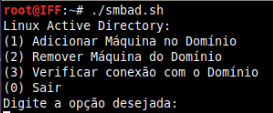
\includegraphics{figuras/smbad}}
   	\caption{Tela do script para inserir maquinas linux no AD}
    \label{smbad}
\end{figure}

\section{Windows no domínio Samba 4}